\chapter{Diagrams modelisation}

In order to produce a visual schema from a SpinalHDL program, we need to parse his AST and produce an intermediate model for the diagrams. The reason to use an intermediate model is that we could then build multiple backend generator for multiple output target. The completeme pipeline of the generation is visible in figure \ref{fig:generation-pipeline}.

\begin{figure}[h] % {{{ figure
    \centering
    \fbox{
        \digraph[scale=0.5]{GenerationPipeline}{
            node [shape=record];
            graph [rankdir=LR,
                   ranksep="1",
                   nodesep="1"];
            S [label="SpinalHDL"];
            I [label="Intermediate model"]
            S -> I;
            I -> JSON;
            I -> dot;
        }
    }
    \caption[KlugHDL generation pipeline]{This figure show the entire generation pipeline use by KlugHDL in order to generate different output. The intermediate model is use to produce the target code, for example dot or JSON file}
    \label{private def generateComponent(diagram : Diagram) : Model = {
    // add all the children of the parent to the diagrams
    diagram.foreachChildren(diagram.addComponents, topLevel)
    // add the input and output parent connection, except it's top level
    if (diagram.parent != null)
      diagram.addIoComponents(diagram.parent)
    this
  }}
\end{figure} % }}}

We also need to introduce an crucial element to understand how the model is build : the hierarchy visualisation.

\section{Hierarchy visualisation}

The diagrams produces by KlugHDL are kind of special, they are hierarchical ones. That's means we need to find a way to show the hierarchy between the components of a SpinalHDL program. There is multiple way to do this :
\begin{itemize}
  \item Showing the elements using a hierarchical layout, like in family tree
  \item Showing the elements one by one (multiple diagrams)
  \item Showing the elements using a tree view, like in file explorer
  \item Showing the elements in 3D, the brothers at the same height and the parents higher
\end{itemize}

\subsection{Hierarchical layout}

The hierarchical layout is the simplest way to achieve the visualisation of the hierarchy. The figure \ref{fig:hierarchical-layout-simple} illustrate a simple hierarchical layout with some children and parent.

\begin{figure}
  \centering
  \fbox{
    \digraph[scale=0.5]{SimpleHierarchicalLayout}{
        node [shape=record];
        graph [ranksep="1",
               nodesep="1"];
        A1 [label="{{<a> io.a | <b> io.b}|RandomComponent|{<c> io.c|<d> io.d}}"];

        B1 [label="{{<a> io.a | <b> io.b}|AndGate|{<c> io.c}}"];
        B2 [label="{{<a> io.a | <b> io.b}|AndXorGate|{<c> io.c|<d> io.d}}"];
        B3 [label="{{<a> io.a | <b> io.b}|OrGate|{<c> io.c}}"];

        C1 [label="{{<a> io.a | <b> io.b}|AndGate|{<c> io.c}}"];
        C2 [label="{{<a> io.a | <b> io.b}|XorGate|{<c> io.c}}"];

        A1:a -> B1:a;
        A1:b -> B1:b;
        A1:a -> B2:a;
        A1:b -> B2:b;
        A1:a -> B3:a;
        A1:b -> B3:b;

        B2:a -> C1:a;
        B2:a -> C2:a;
        B2:b -> C1:b;
        B2:b -> C2:a;

        C1:c -> B2:c;
        C2:c -> B2:c;

        B2:c -> A1:c;
        B1:c -> A1:d;
        B3:c -> A1:d;
    }
  }
  \caption[Simple hierarchical layout for diagram visualization]{The simplest hierarchical visualization}
  \label{fig:hierarchical-layout-simple}
\end{figure}

\section{A visual example}

The diagram we want to produce, as explain in \ref{sec:graph-layout}, ownes the following property :
\begin{itemize}
  \item Oriented
  \item Cyclic
  \item Connection between port on nodes and not between nodes
\end{itemize}

\begin{figure}[h]
  \centering
  \fbox{
  \digraph[scale=0.5]{DiagramExample}{
          graph [rankdir=LR,ranksep="2",nodesep="2"];
          node [shape=record];
          AndGate [label="{{<iob>iob | <ioa>ioa}|AndGate|{<ioc>ioc}}"];
          OrGate [label="{{<ioa>ioa | <iob>iob}|OrGate|{<ioc>ioc}}"];
          EXTERNAL_INPUT [label="{EXTERNAL_INPUT|{<ioa>ioa | <iob>iob}}"];
          EXTERNAL_OUTPUT [label="{{<ioc>ioc}|EXTERNAL_OUTPUT}"];
             EXTERNAL_INPUT:ioa -> AndGate:ioa;
          EXTERNAL_INPUT:ioa -> OrGate:ioa;
          EXTERNAL_INPUT:iob -> OrGate:iob;
          EXTERNAL_INPUT:iob -> AndGate:iob;OrGate:ioc -> EXTERNAL_OUTPUT:ioc;
          AndGate:ioc -> EXTERNAL_OUTPUT:ioc;
        }
  }
  \caption[Complete example of a KlugHDL diagram]{A complete example of a KlugHDL diagram, with connection between ports and oriented edges. The EXTERNAL\_INPUT and EXTERNAL\_OUTPUT are the interface of the component}
  \label{fig:example-spinal-diag}
\end{figure}

\section{Model representation}

The model representation is builded using the oriented-object paradigm, the figure \ref{fig:model-class-diagram} show the class diagram of the models.

\begin{figure}[h]
  \centering
  \fbox{
  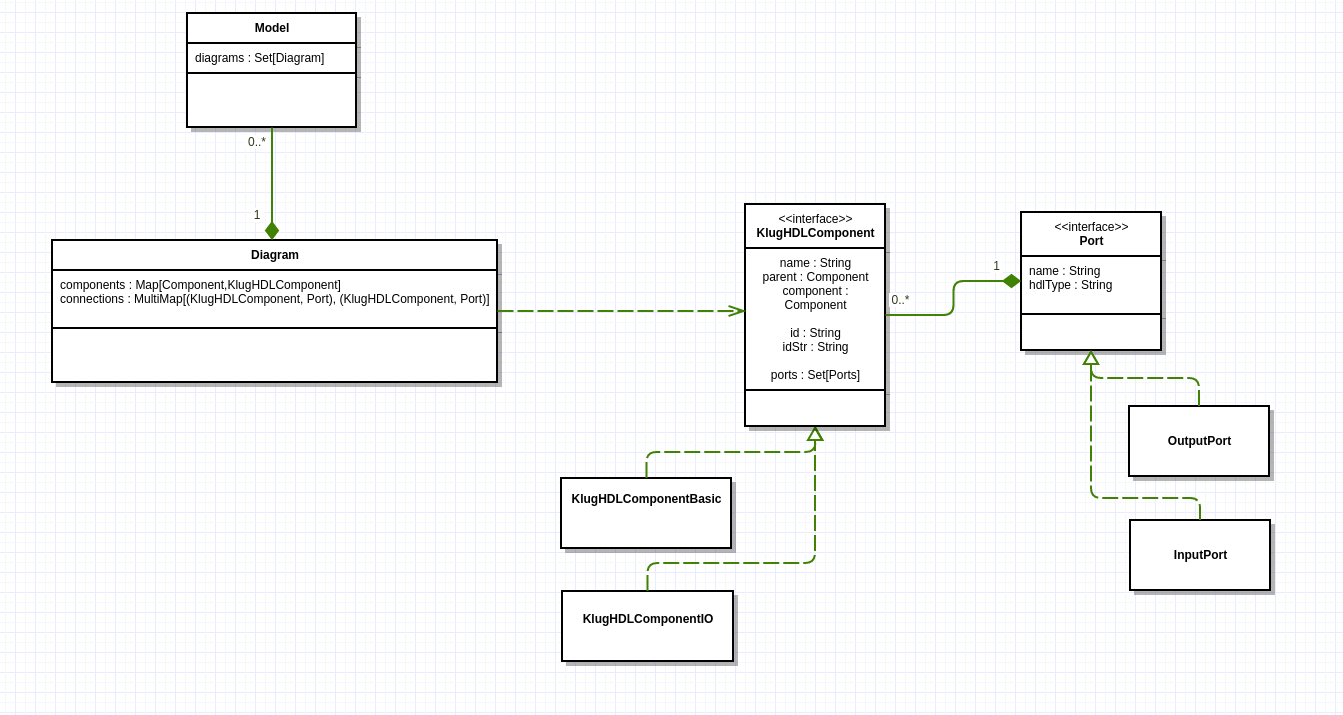
\includegraphics[width=0.99\textwidth]{img/class-diagram-intermeditate-model}
  }
  \caption[Class diagram of the intermediate model]{The complete class diagram of the intermediate model representation}
  \label{fig:model-class-diagram}
\end{figure}

\section{Conclusion}

The major advantages of such an intermediate representation is the capability to evolve the program in order to produce additionnal output. For now there is just a \textbf{dot} and \textbf{JSON} backend. It's also provide a way to check the correctness of the diagram after the parsing on the AST : connections with non-existing port for example.
